\section{Results}

For running the application the following commands were used for compiling,
uploading the project and monitoring the port to observe the periodic reports.

\begin{verbatim}
# list connected boards and their ports
pio device list
# compile and upload to ESP32
pio run --target upload
# open serial monitor at 115200 baud
pio device monitor --baud 115200
\end{verbatim}

Below is the output of the commands listed above

\begin{verbatim}
======================================
  Lab 6 - Analog Signal Acquisition
======================================
Sensor    : DHT11 (digital) GPIO4
Acq.period: 2000 ms
Pipeline  : Saturation -> Median(5) -> EMA(a=0.20)
Thresholds: ON >= 28.0C, OFF <= 24.0C
Display   : OLED 128x64 SSD1306 + LCD 20x4 + Serial
======================================

>raw:24.00,median:24.00,ema:24.00,thresh_high:28.0,thresh_low:24.0
>raw:24.00,median:24.00,ema:24.00,thresh_high:28.0,thresh_low:24.0
>raw:25.00,median:24.00,ema:24.00,thresh_high:28.0,thresh_low:24.0

===== SENSOR REPORT (t=5000 ms) =====
Active sensor : DHT11
Validity      : OK
Raw           : 25.00 C
Saturated+Med : 24.00 C  (median window=5)
EMA averaged  : 24.00 C  (alpha=0.20)
Alert         : OFF  (thresholds: ON>=28.0 OFF<=24.0)
====================================

>raw:29.00,median:25.00,ema:24.20,thresh_high:28.0,thresh_low:24.0
>raw:30.00,median:29.00,ema:25.16,thresh_high:28.0,thresh_low:24.0
>raw:30.00,median:30.00,ema:26.13,thresh_high:28.0,thresh_low:24.0

===== SENSOR REPORT (t=10000 ms) =====
Active sensor : DHT11
Validity      : OK
Raw           : 30.00 C
Saturated+Med : 30.00 C  (median window=5)
EMA averaged  : 27.10 C  (alpha=0.20)
Alert         : ON  (thresholds: ON>=28.0 OFF<=24.0)
====================================
\end{verbatim}

The system behavior is as follows:
\begin{itemize}
  \item At startup, the OLED shows \texttt{Lab6 SigAcquire} / \texttt{Starting...}
    for 1\,second while all modules initialize.
  \item During normal operation (temperature below $28\,^\circ$C), the \textbf{green LED}
    is on and the OLED displays all pipeline stages: raw temperature, median-filtered
    value, and EMA-averaged value, along with the sensor name and alert state.
  \item The serial plotter line in \texttt{>name:value} format allows real-time
    visualization in the VS Code Serial Plotter extension, where the raw, median, and
    EMA traces can be compared side by side against the threshold reference lines.
  \item When the temperature rises above $28\,^\circ$C (as seen by the median-filtered
    value), the alert transitions to ON: the \textbf{red LED} turns on, the green LED
    turns off, and the OLED display updates to show \texttt{Alert: ON}.
  \item The alert turns OFF only after the median-filtered temperature drops below
    $24\,^\circ$C, preventing chattering in the $24$--$28\,^\circ$C hysteresis band.
  \item The EMA trace on the serial plotter visibly lags behind the raw and median
    traces, demonstrating the smoothing effect of the weighted average with
    $\alpha = 0.2$.
  \item Every 500\,ms, a serial plotter data line is emitted. Every 5\,seconds, a full
    structured report is printed showing the active sensor, validity, all pipeline
    values with their parameters, and alert configuration.
\end{itemize}

\clearpage
Below is the visual representation of the circuit

\begin{figure}[h]
    \centering
    
\includegraphics[width=0.6\textwidth]{img/ledoff.jpg}
    \caption{Circuit in working state}
    \label{fig:ledoff}
\end{figure}

Figure \ref{fig:ledoff} shows the circuit in its idle state with both LEDs off before
acquisition begins.

\clearpage
This is how the plotting of values in time look:

\begin{figure}[h]
    \centering
    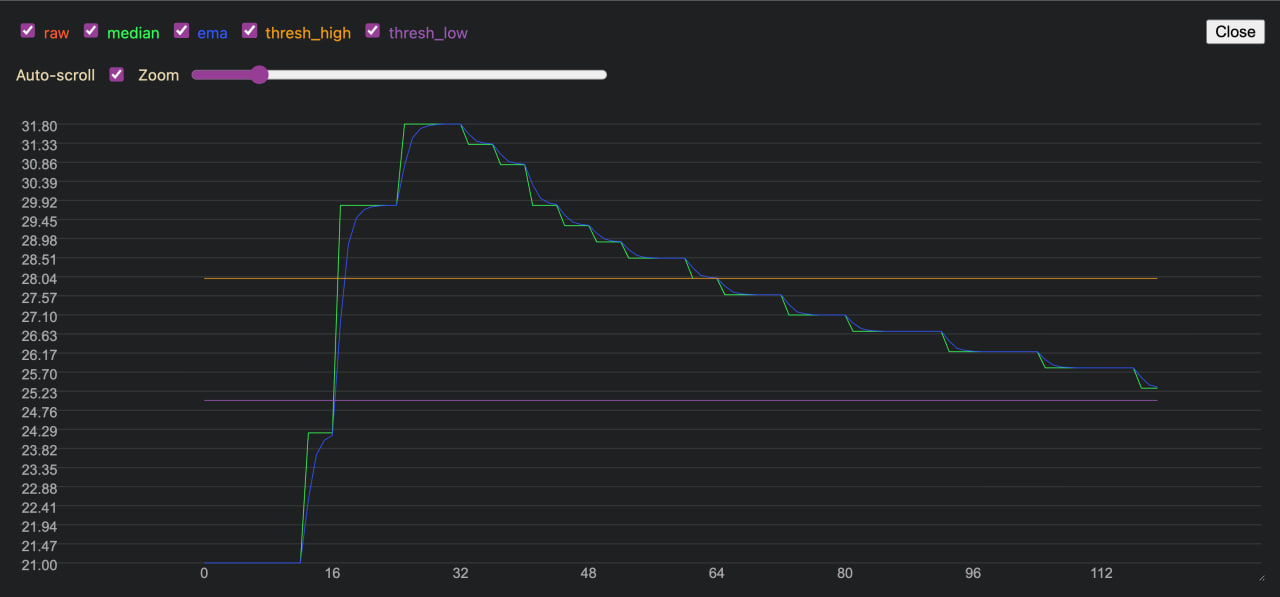
\includegraphics[width=1\textwidth]{img/plot.jpg}
    \caption{Ploting the sensor values and filtered data}
    \label{fig:plot}
\end{figure}
